\documentclass[aspectratio=169,10pt]{beamer}

\usetheme{metropolis}
\usepackage[utf8]{inputenc}
\usepackage[T1]{fontenc}
\usepackage{tikz}
\usetikzlibrary{arrows,positioning}
\usetikzlibrary{decorations.pathreplacing,calc}
\usetikzlibrary{arrows.meta,positioning,shadows}
\usepackage{xcolor}
\usepackage{transparent}
\usepackage{graphicx}

% =========================================================
% COLORS
% =========================================================
\definecolor{pdblue}{RGB}{31,119,180}
\definecolor{pdorange}{RGB}{255,127,130}
\definecolor{pdgreen}{RGB}{44,160,44}
\definecolor{pdred}{RGB}{214,39,40}
\definecolor{pdpurple}{RGB}{148,103,189}
\definecolor{pdnavy}{RGB}{23,42,58}
\definecolor{pdfooter}{RGB}{174,195,204}
\definecolor{pdCream}{HTML}{F1F4F8}
\definecolor{pdGrayText}{HTML}{4A4A4A}

% =========================================================
% THEME
% =========================================================
\setbeamercolor{palette primary}{bg=pdnavy,fg=white}
\setbeamercolor{frametitle}{bg=pdnavy,fg=white}
\setbeamercolor{normal text}{fg=pdnavy}
\setbeamercolor{alerted text}{fg=pdred}
\setbeamercolor{example text}{fg=pdgreen}
\setbeamercolor{title separator}{fg=pdorange}
\setbeamercolor{progress bar}{fg=pdorange,bg=pdnavy!15}

\metroset{
    progressbar=frametitle,
    numbering=fraction,
    block=fill,
    sectionpage=none
}
\setbeamertemplate{navigation symbols}{}

% =========================================================
% FOOTER
% =========================================================
\setbeamertemplate{footline}{
\begin{tikzpicture}[remember picture,overlay]
    \fill[pdnavy]
        (current page.south west)
        rectangle
        ([yshift=4.4ex]current page.south east);

    \draw[pdfooter!55,line width=.8pt]
        ([yshift=4.4ex]current page.south west) --
        ([yshift=4.4ex]current page.south east);

    \node[anchor=south west,xshift=.8em,yshift=.8ex,
          text=white,font=\tiny\bfseries]
        at (current page.south west)
        {Tajrian \textcolor{pdfooter}{\textbullet} CSE, BUET};

    \node[anchor=south,yshift=.8ex,text=pdfooter,
          font=\scriptsize\itshape]
        at (current page.south)
        {Participatory Design};

    \node[anchor=south east,xshift=-.8em,yshift=.75ex,
          fill=pdfooter,rounded corners=1.5pt,inner sep=2.5pt,
          text=pdnavy,font=\scriptsize\bfseries]
        at (current page.south east)
        {\insertframenumber\,/\,\inserttotalframenumber};
\end{tikzpicture}
}

% =========================================================
% TIKZ STYLES
% =========================================================
\tikzset{
    card/.style={
        draw=#1,thick,rounded corners=5pt,fill=#1!10,
        align=center,text=pdnavy,drop shadow
    },
    card/.default=pdblue,
    pill/.style={
        draw=#1,thick,rounded corners=9pt,fill=#1!12,
        align=center,font=\scriptsize\bfseries,text=pdnavy
    },
    pill/.default=pdblue,
    arrow/.style={
        -{Latex[length=2.5mm]},thick,draw=pdnavy!75
    }
}

\begin{document}

% =========================================================
% 1. TITLE
% =========================================================
\begin{frame}[plain]
\begin{tikzpicture}[remember picture,overlay]

\fill[pdnavy]
(current page.south west) rectangle (current page.north east);

\node[
anchor=north west,
text=white,
align=left
] at ([xshift=1.3cm,yshift=-1.5cm]current page.north west)
{
{\color{pdorange}\bfseries REAL-WORLD SYNTHESIS}\\[20pt]
{\Huge\bfseries Participatory Design in Practice}
};

\draw[pdfooter!18]
([yshift=-1.2cm]current page.north west) --
([yshift=-1.2cm]current page.north east);

\begin{scope}[shift={([yshift=-1cm]current page.center)}]
\draw[pdfooter!35,line width=1.5pt] (-5,0)--(5,0);

\foreach \x/\n in {-3.75/1,-1.25/2,1.25/3,3.75/4}{
\node[
circle,fill=pdorange,draw=white,thick,
minimum size=19pt,inner sep=0pt
] at (\x,0)
{\tiny\bfseries\color{pdnavy}\n};
}

\node[text=white,font=\scriptsize\bfseries] at (-3.75,-.55)
{APPLICATIONS};
\node[text=white,font=\scriptsize\bfseries] at (-1.25,-.55)
{BENEFITS};
\node[text=white,font=\scriptsize\bfseries] at (1.25,-.55)
{CHALLENGES};
\node[text=white,font=\scriptsize\bfseries] at (3.75,-.55)
{CONCLUSION};
\end{scope}

\node[
anchor=south west,
xshift=1.3cm,
yshift=.55cm,
text=pdfooter,
font=\tiny
] at (current page.south west)
{
2305082 \quad\textcolor{pdorange}{\textbullet}\quad
Tajrian Shams Sneha
};

\end{tikzpicture}
\end{frame}
% =========================================================
% 2. FROM PROCESS TO PRACTICE
% =========================================================
\begin{frame}{From Usage to Challenges}
\centering

\vspace{.3cm}


\begin{tikzpicture}[node distance=1cm]

\node[pill=pdorange,minimum width=3.1cm,minimum height=.75cm]
(where){\normalsize WHERE?\\[2pt]\small Applications};

\node[pill=pdgreen,minimum width=3.1cm,minimum height=.75cm,
right=of where]
(why){\normalsize WHY?\\[2pt]\small Benefits};

\node[pill=pdred,minimum width=3.1cm,minimum height=.75cm,
right=of why]
(catch){\normalsize WHAT'S THE CATCH?\\[2pt]\small Challenges};

\draw[arrow](where)--(why);
\draw[arrow](why)--(catch);

\end{tikzpicture}

\vspace{.8cm}

{\Large\bfseries
Participatory Design matters because\\
it changes who gets to shape the system.}

\vspace{.4cm}

{\small\color{pdGrayText}
Where does it work, what does it add,
and where does participation become difficult?
}

\end{frame}

% =========================================================
% 3. APPLICATIONS
% =========================================================
\begin{frame}{Applications: Where Does PD Show Up?}
\centering

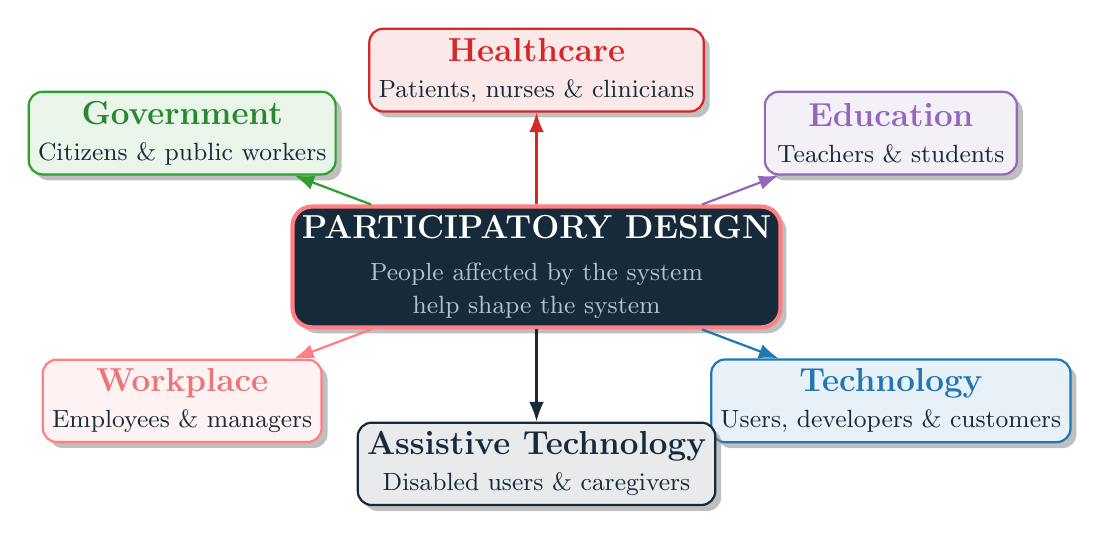
\begin{tikzpicture}[node distance=1cm]

\node[
draw=pdorange,line width=1.5pt,rounded corners=7pt,
fill=pdnavy,minimum width=4cm,minimum height=1.4cm,
align=center,text=white,drop shadow
](core) at (0,0)
{
{\large\bfseries PARTICIPATORY DESIGN}\\[3pt]
{\small\color{pdfooter}People affected by the system}\\
{\small\color{pdfooter}help shape the system}
};

\transparent{0.5}\node[card=pdred,minimum width=3.2cm,minimum height=1.05cm]
(health) at (0,2.5)
{\bfseries\color{pdred}\large Healthcare\\[1pt]
\small Patients, nurses \& clinicians};

\node[card=pdpurple,minimum width=3.2cm,minimum height=1.05cm]
(edu) at (4.5,1.7)
{\bfseries\color{pdpurple}\large Education\\[1pt]
\small Teachers \& students};

\node[card=pdgreen,minimum width=3.2cm,minimum height=1.05cm]
(gov) at (-4.5, 1.7)
{\bfseries\color{pdgreen!80!pdnavy}\large Government\\[1pt]
\small Citizens \& public workers};

\node[card=pdblue,minimum width=3.2cm,minimum height=1.05cm]
(tech) at (4.5,-1.7)
{\bfseries\color{pdblue}\large Technology\\[1pt]
\small Users, developers \& customers};

\node[
card=pdorange,
minimum width=3.2cm,
minimum height=1.0cm
] (wp) at (-4.5,-1.7)
{\bfseries\color{pdorange!90!pdnavy}\large Workplace\\[1pt]
\small Employees \& managers};

\node[
card=pdnavy,
minimum width=3.2cm,
minimum height=1.0cm
](atech) at (0,-2.5)
{\bfseries\large Assistive Technology\\[1pt]
\small Disabled users \& caregivers};

\draw[arrow,pdred](core)--(health);
\draw[arrow,pdpurple](core)--(edu);
\draw[arrow,pdgreen](core)--(gov);
\draw[arrow,pdblue](core)--(tech);
\draw[arrow,pdorange](core)--(wp);
\draw[arrow,pdnavy](core)--(atech);

\end{tikzpicture}

\vspace{.15cm}

\end{frame}

% =========================================================
% 4. APPLICATION EXAMPLES
% =========================================================
\begin{frame}{Application Lens: Real Context Matters}
\centering

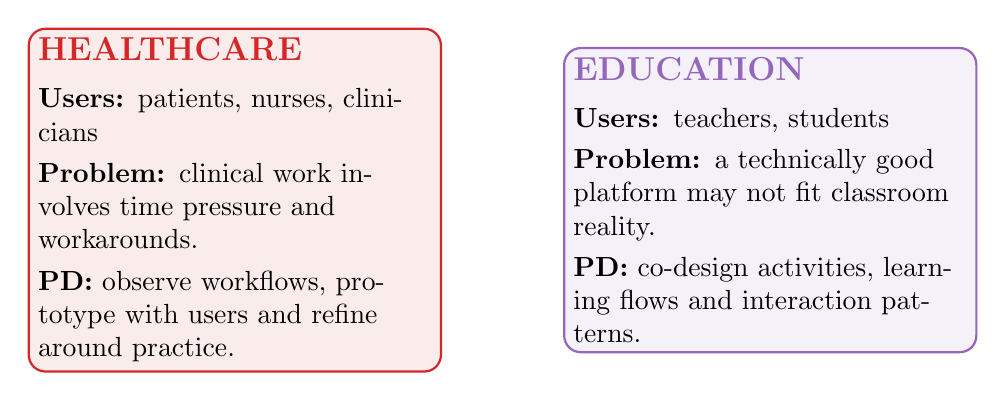
\begin{tikzpicture}

\node[
draw=pdred,thick,rounded corners=6pt,fill=pdred!9,
text width=5cm,minimum height=3.4cm,align=left
] at (-3.4,0)
{
{\large\bfseries\color{pdred}HEALTHCARE}\\[5pt]
\textbf{Users:} patients, nurses, clinicians\\[3pt]
\textbf{Problem:} clinical work involves
time pressure and workarounds.\\[3pt]
\textbf{PD:} observe workflows, prototype
with users and refine around practice.
};

\node[
draw=pdpurple,thick,rounded corners=6pt,fill=pdpurple!9,
text width=5cm,minimum height=3.4cm,align=left
] at (3.4,0)
{
{\large\bfseries\color{pdpurple}EDUCATION}\\[5pt]
\textbf{Users:} teachers, students\\[3pt]
\textbf{Problem:} a technically good platform
may not fit classroom reality.\\[3pt]
\textbf{PD:} co-design activities,
learning flows and interaction patterns.
};

\end{tikzpicture}

\vspace{.35cm}

{\small\color{pdGrayText}
The value is not simply asking users what they want;
it is learning how the system fits into real life.
}
\end{frame}

% =========================================================
% 5. APPLICATION DETAILS
% =========================================================
\begin{frame}{Six Domains, One Principle}
\centering

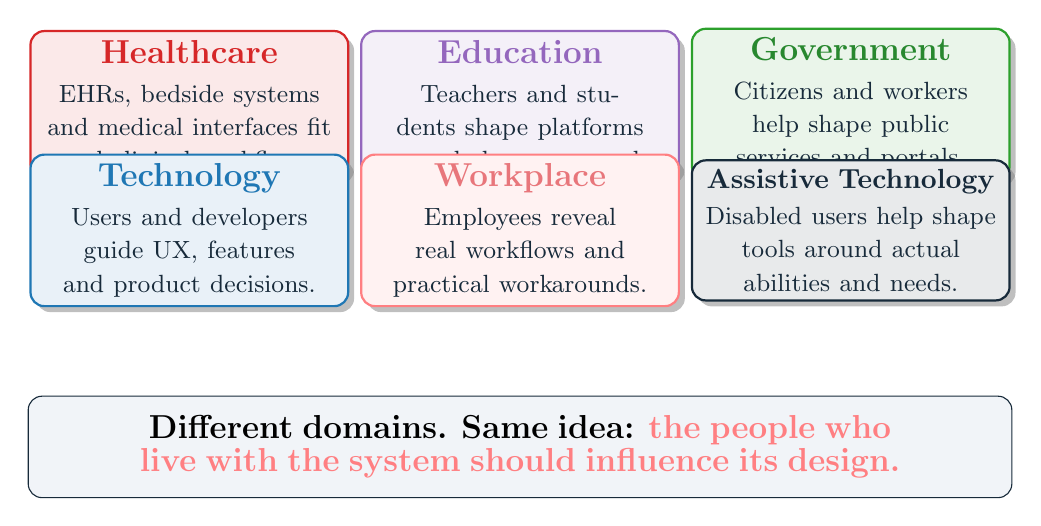
\begin{tikzpicture}[x=1cm,y=1cm]

\node[card=pdred,text width=3.8cm,minimum height=1.25cm]
at (-4.2,1.35)
{\textbf{\color{pdred}\large Healthcare}\\[2pt]
\small EHRs, bedside systems and medical interfaces
fit real clinical workflows.};

\node[card=pdpurple,text width=3.8cm,minimum height=1.25cm]
at (0,1.35)
{\textbf{\color{pdpurple}\large Education}\\[2pt]
\small Teachers and students shape platforms
around classroom needs.};

\node[card=pdgreen,text width=3.8cm,minimum height=1.25cm]
at (4.2,1.35)
{\textbf{\color{pdgreen!80!pdnavy}\large Government}\\[2pt]
\small Citizens and workers help shape
public services and portals.};

\node[card=pdblue,text width=3.8cm,minimum height=1.25cm]
at (-4.2,-.25)
{\textbf{\color{pdblue}\large Technology}\\[2pt]
\small Users and developers guide UX,
features and product decisions.};

\node[card=pdorange,text width=3.8cm,minimum height=1.25cm]
at (0,-.25)
{\textbf{\color{pdorange!90!pdnavy}\large Workplace}\\[2pt]
\small Employees reveal real workflows
and practical workarounds.};

\node[card=pdnavy,text width=3.8cm,minimum height=1.25cm]
at (4.2,-.25)
{\textbf{\normalsize Assistive Technology}\\[1pt]
\small Disabled users help shape tools
around actual abilities and needs.};

\node[
draw=pdnavy,fill=pdCream,rounded corners=5pt,
text width=12cm,align=center,inner sep=7pt
] at (0,-3)
{\large\bfseries
Different domains. Same idea:
\textcolor{pdorange}{\large the people who live with the system
should influence its design.}};

\end{tikzpicture}
\end{frame}


% =========================================================
% 6. BENEFITS
% =========================================================
\begin{frame}{Benefits: Why Bring People Into the Process?}
\centering

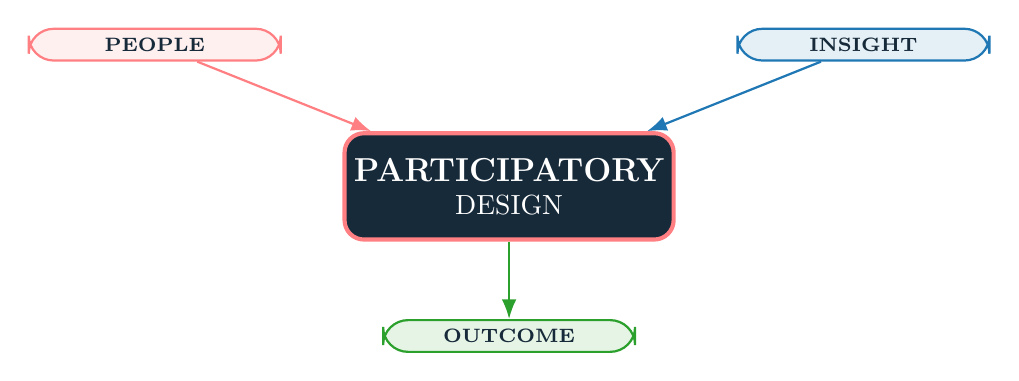
\begin{tikzpicture}

\node[
draw=pdorange,line width=1.5pt,rounded corners=7pt,
fill=pdnavy,minimum width=4cm,minimum height=1.35cm,
align=center,text=white
](pd) at (0,0)
{\large\bfseries PARTICIPATORY\\DESIGN};

\node[pill=pdorange,minimum width=3.2cm]
(people) at (-4.5,1.8){PEOPLE};

\node[pill=pdblue,minimum width=3.2cm]
(insight) at (4.5,1.8){INSIGHT};

\node[pill=pdgreen,minimum width=3.2cm]
(outcome) at (0,-1.9){OUTCOME};

\draw[arrow,pdorange](people)--(pd);
\draw[arrow,pdblue](insight)--(pd);
\draw[arrow,pdgreen](pd)--(outcome);

\end{tikzpicture}

\vspace{.3cm}

{\normalsize\color{pdGrayText}
Three layers explain most of the value:
\textbf{\normalsize who participates, what they reveal, and what the design becomes.}
}
\end{frame}

% =========================================================
% 7.1 PEOPLE + INSIGHT + OUTCOME
% =========================================================
\begin{frame}{The Co-Creation Equation}
\centering

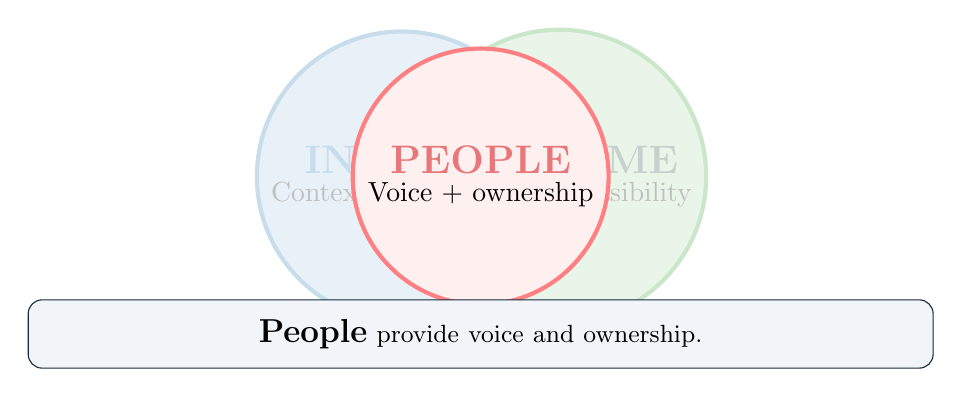
\begin{tikzpicture}


\node[
circle,draw=pdgreen!25,line width=1.5pt,fill=pdgreen!10,
minimum size=2.7cm,align=center
](o) at (1,0)
{\Large\bfseries\color{pdgreen!25!pdnavy!25}OUTCOME\\[-2pt]
\normalsize\color{black!25} Usability + feasibility};

\node[
circle,draw=pdblue!25,line width=1.5pt,fill=pdblue!10,
minimum size=2.7cm,align=center
](i) at (-1,0)
{\Large\bfseries\color{pdblue!25}INSIGHT\\[-2pt]
\normalsize\color{black!25} Context + knowledge};

\node[
circle,draw=pdorange,line width=1.5pt,fill=pdorange!12,
minimum size=2.7cm,align=center
](p) at (0,0)
{\Large\bfseries\color{pdorange!90!pdnavy}PEOPLE\\[-2pt]
\normalsize Voice + ownership};


\node[
draw=pdnavy,fill=pdCream,rounded corners=5pt,
text width=11cm,align=center,inner sep=7pt
] at (0,-2)
{\small
\textbf{\large People} provide voice and ownership.};

\end{tikzpicture}
\end{frame}

% =========================================================
% 7.2 PEOPLE + INSIGHT + OUTCOME
% =========================================================
\begin{frame}{The Co-Creation Equation}
\centering

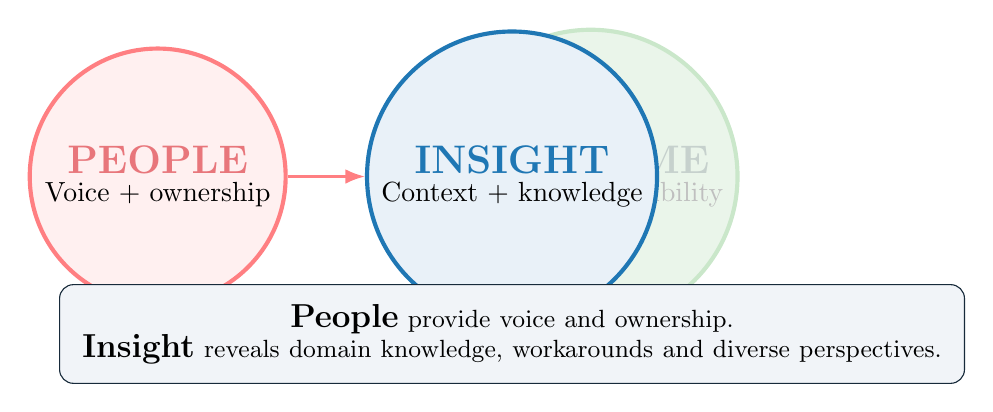
\begin{tikzpicture}

\node[
circle,draw=pdorange,line width=1.5pt,fill=pdorange!12,
minimum size=2.7cm,align=center
](p) at (-4.5,0)
{\Large\bfseries\color{pdorange!90!pdnavy}PEOPLE\\[-2pt]
\normalsize Voice + ownership};

\node[
circle,draw=pdgreen!25,line width=1.5pt,fill=pdgreen!10,
minimum size=2.7cm,align=center
](o) at (1,0)
{\Large\bfseries\color{pdgreen!25!pdnavy!25}OUTCOME\\[-2pt]
\normalsize\color{black!25} Usability + feasibility}; 

\node[
circle,draw=pdblue,line width=1.5pt,fill=pdblue!10,
minimum size=2.7cm,align=center
](i) at (0,0)
{\Large\bfseries\color{pdblue}INSIGHT\\[-2pt]
\normalsize Context + knowledge};


\draw[arrow,pdorange](p)--(i);


\node[
draw=pdnavy,fill=pdCream,rounded corners=5pt,
text width=11cm,align=center,inner sep=7pt
] at (0,-2)
{\small
\textbf{\large People} provide voice and ownership.\\
\textbf{\large Insight} reveals domain knowledge, workarounds
and diverse perspectives.\\
};

\end{tikzpicture}
\end{frame}

% =========================================================
% 7.3 PEOPLE + INSIGHT + OUTCOME
% =========================================================
\begin{frame}{The Co-Creation Equation}
\centering

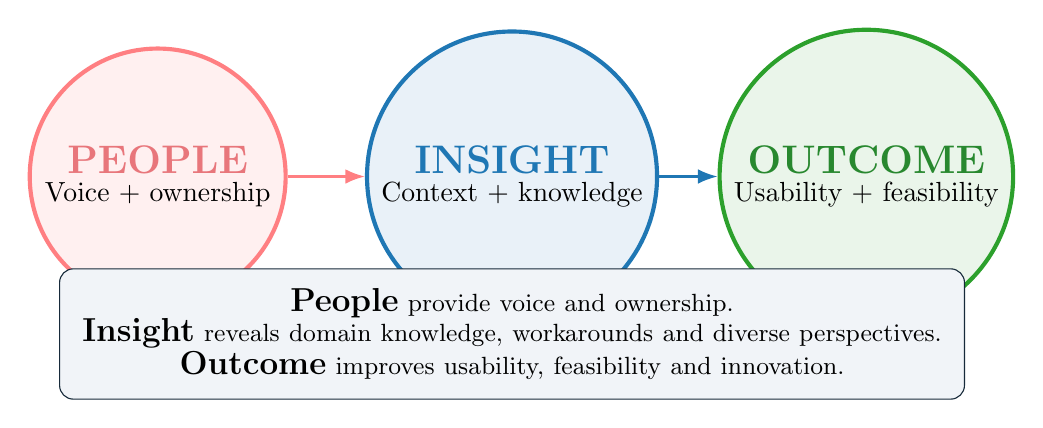
\begin{tikzpicture}

\node[
circle,draw=pdorange,line width=1.5pt,fill=pdorange!12,
minimum size=2.7cm,align=center
](p) at (-4.5,0)
{\Large\bfseries\color{pdorange!90!pdnavy}PEOPLE\\[-2pt]
\normalsize Voice + ownership};

\node[
circle,draw=pdblue,line width=1.5pt,fill=pdblue!10,
minimum size=2.7cm,align=center
](i) at (0,0)
{\Large\bfseries\color{pdblue}INSIGHT\\[-2pt]
\normalsize Context + knowledge};

\node[
circle,draw=pdgreen,line width=1.5pt,fill=pdgreen!10,
minimum size=2.7cm,align=center
](o) at (4.5,0)
{\Large\bfseries\color{pdgreen!80!pdnavy}OUTCOME\\[-2pt]
\normalsize Usability + feasibility};

\draw[arrow,pdorange](p)--(i);
\draw[arrow,pdblue](i)--(o);

\node[
draw=pdnavy,fill=pdCream,rounded corners=5pt,
text width=11cm,align=center,inner sep=7pt
] at (0,-2)
{\small
\textbf{\large People} provide voice and ownership.\\
\textbf{\large Insight} reveals domain knowledge, workarounds
and diverse perspectives.\\
\textbf{\large Outcome} improves usability, feasibility and innovation.
};

\end{tikzpicture}
\end{frame}

% =========================================================
% 8. CO-CREATION EQUATION
% =========================================================
\begin{frame}{Benefits: People $\rightarrow$ Insight $\rightarrow$ Outcome}
\centering

\resizebox{0.95\linewidth}{!}{%
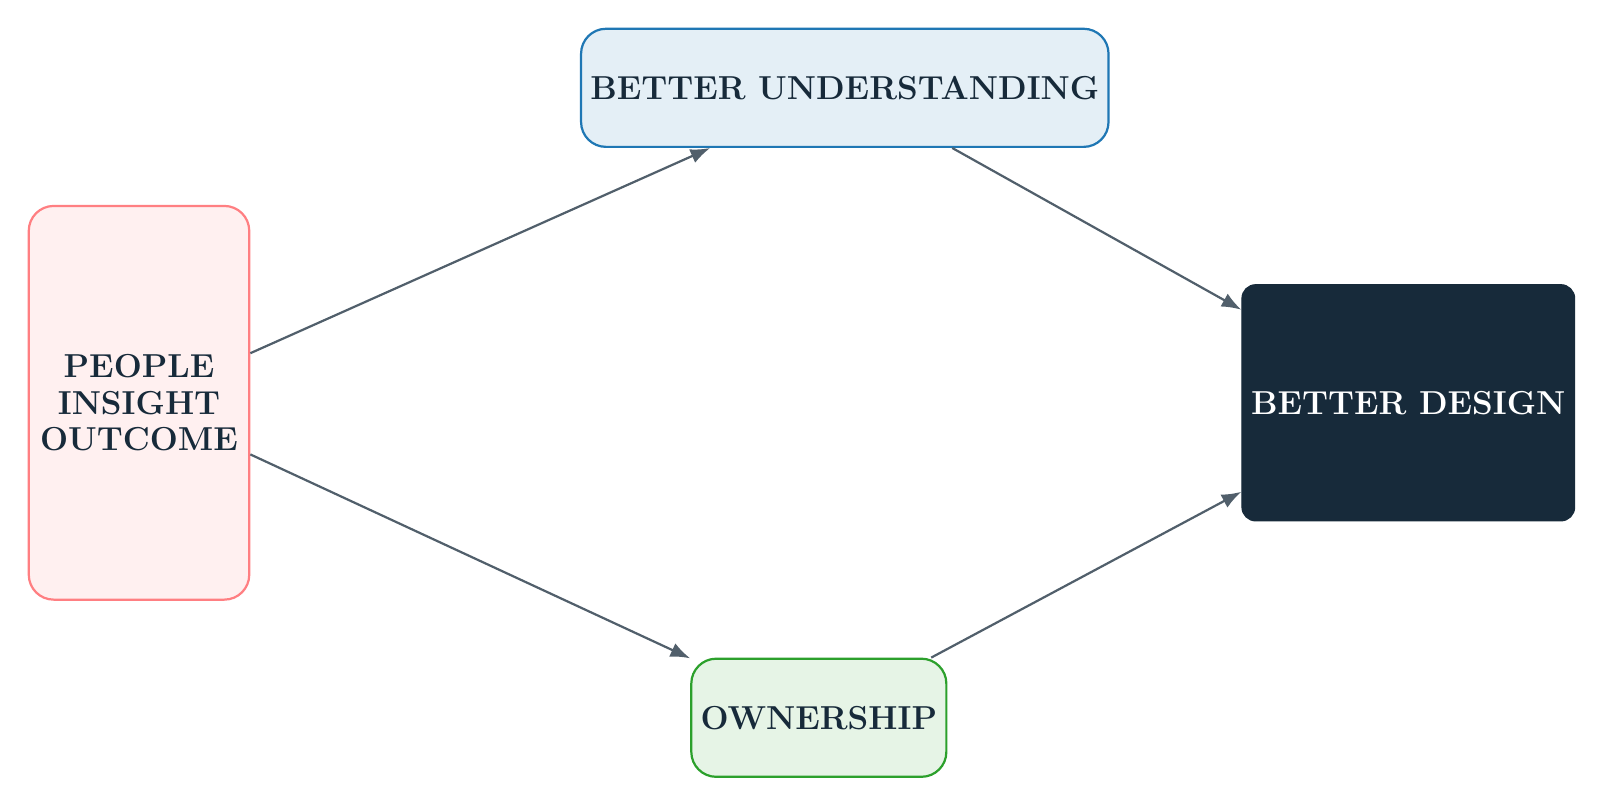
\begin{tikzpicture}

\node[pill=pdorange,minimum width=2.8cm,minimum height=5cm]
(p) at (-6,0){\large PEOPLE\\[4 pt]
\large INSIGHT\\[4 pt]
\large OUTCOME};

\node[pill=pdblue,minimum width=2.8cm,minimum height=1.5cm,
right=1cm of p]
(i) at (-1.4,4){\large BETTER UNDERSTANDING};

\node[pill=pdgreen,minimum width=2.8cm,minimum height=1.5cm,
right=1cm of i]
(o) at (0,-4){\large OWNERSHIP};

\node[
draw=pdnavy,fill=pdnavy,text=white,rounded corners=5pt,
minimum width=3.4cm,minimum height=3cm,
right=1cm of o,align=center
]
(b) at (7, 0){\large\bfseries BETTER DESIGN};

\draw[arrow](p)--(i);
\draw[arrow](p)--(o);
\draw[arrow](i)--(b);
\draw[arrow](o)--(b);



\end{tikzpicture}%
}
\end{frame}

% =========================================================
% 9. DREYFUSS
% =========================================================
\begin{frame}{Why Collaboration Is at the Heart of It}
\centering

\vspace{.35cm}

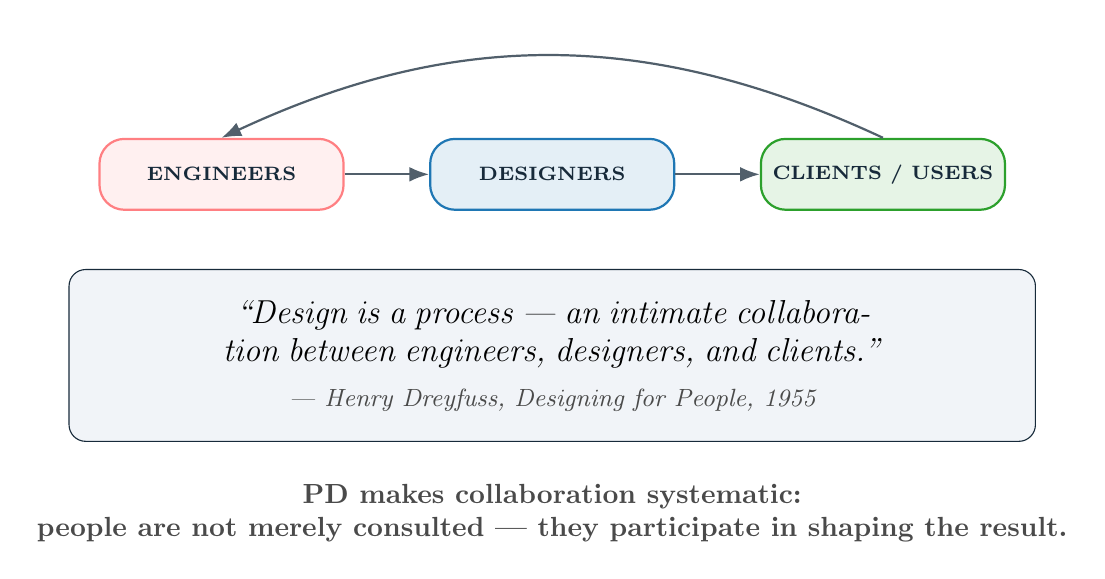
\begin{tikzpicture}

\node[pill=pdorange,minimum width=3.1cm,minimum height=0.9cm]
(eng) at (-4.2,2.3){ENGINEERS};

\node[pill=pdblue,minimum width=3.1cm, minimum height=.9cm]
(des) at (0,2.3){DESIGNERS};

\node[pill=pdgreen,minimum width=3.1cm, minimum height=.9cm]
(cli) at (4.2,2.3){CLIENTS / USERS};

\draw[arrow](eng)--(des);
\draw[arrow](des)--(cli);
\draw[arrow] (cli.north) to[bend right=25] (eng.north);

\node[
draw=pdnavy,rounded corners=6pt,fill=pdCream,
text width=11.5cm,align=center,inner sep=11pt
] at (0,0)
{
\large\itshape
``Design is a process --- an intimate collaboration
between engineers, designers, and clients.''\\[4pt]
{\small\color{pdGrayText}
--- Henry Dreyfuss, \textit{Designing for People}, 1955}
};

\node[
font=\normalsize\bfseries,text=pdGrayText,align=center
] at (0,-2)
{
PD makes collaboration systematic:\\
people are not merely consulted ---
they participate in shaping the result.
};

\end{tikzpicture}
\end{frame}

% =========================================================
% 10. CHALLENGE DIVIDER
% =========================================================
\begin{frame}[plain]
\begin{tikzpicture}[remember picture,overlay]

\fill[pdred!92!pdnavy]
(current page.south west) rectangle
(current page.north east);

\node[anchor=north west,xshift=1.3cm,yshift=-1.7cm]
at (current page.north west)
{\color{white}\bfseries\small Till now,};

\node[anchor=north west,xshift=1.3cm,yshift=-2.35cm]
at (current page.north west)
{
\begin{minipage}{12.5cm}
{\Huge\bfseries\color{white}Sounds great.}\\[5pt]
{\Huge\bfseries\color{pdorange}So... what's the catch?}
\end{minipage}
};

\begin{scope}[shift={([yshift=-.5cm]current page.center)}]

\node[
circle,draw=pdorange,line width=1.5pt,fill=pdnavy,
minimum size=1.8cm,text=white,align=center
]
(pd) at (3.3,-1.7) {\bfseries PD};

\foreach \x/\y/\t in {
2.5/-.3/TIME,
6.3/0/NEEDS,
-.3/-2/TRUST,
5/-3/DATA}{
\node[
circle,draw=pdfooter!55,fill=pdnavy!65,
minimum size=1cm,text=white,font=\normalsize
] (n-\t) at (\x,\y){\t};
\draw[draw=pdorange,thick](pd)--(n-\t);
}

\end{scope}

\node[anchor=south west,xshift=1.3cm,yshift=.55cm]
at (current page.south west)
{\normalsize\color{pdfooter}
Participation creates value --- but it also creates tensions.};

\end{tikzpicture}
\end{frame}

% =========================================================
% 11. FOUR CHALLENGES
% =========================================================
\begin{frame}{Four Challenges to Manage}
\centering

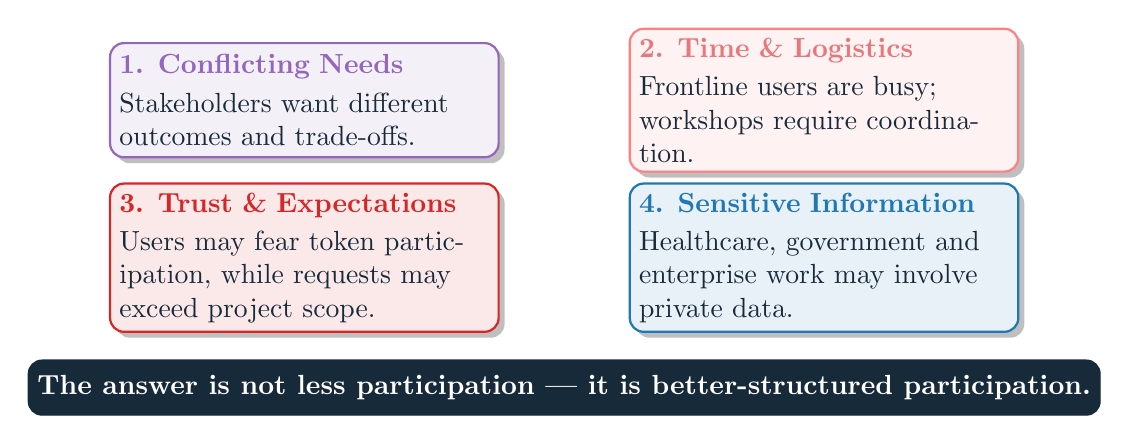
\begin{tikzpicture}

\node[card=pdpurple,text width=4.7cm,minimum height=1.45cm,align=left]
at (-3.3,1.3)
{\textbf{\color{pdpurple}1. Conflicting Needs}\\[2pt]
\normalsize Stakeholders want different outcomes and trade-offs.};

\node[card=pdorange,text width=4.7cm,minimum height=1.45cm,align=left]
at (3.3,1.3)
{\textbf{\color{pdorange!90!pdnavy}2. Time \& Logistics}\\[2pt]
\normalsize Frontline users are busy;
workshops require coordination.};

\node[card=pdred,text width=4.7cm,minimum height=1.45cm,align=left]
at (-3.3,-.7)
{\textbf{\color{pdred}3. Trust \& Expectations}\\[2pt]
\normalsize Users may fear token participation,
while requests may exceed project scope.};

\node[card=pdblue,text width=4.7cm,minimum height=1.45cm,align=left]
at (3.3,-.7)
{\textbf{\color{pdblue}4. Sensitive Information}\\[2pt]
\normalsize Healthcare, government and enterprise
work may involve private data.};

\node[
draw=pdnavy,fill=pdnavy,rounded corners=5pt,
text=white,minimum width=9cm,minimum height=.7cm,
align=center
] at (0,-2.35)
{\normalsize\bfseries
The answer is not less participation ---
it is better-structured participation.};

\end{tikzpicture}
\end{frame}

% =========================================================
% 12. CONFLICT 
% =========================================================
\begin{frame}{Challenges: Conflict....}
\centering

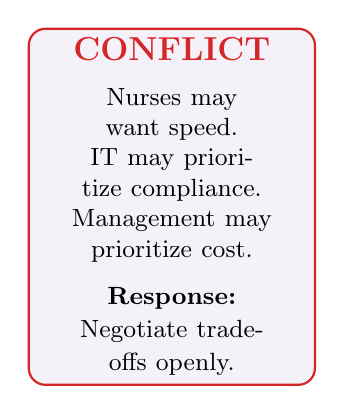
\begin{tikzpicture}

\node[
draw=pdred,thick,rounded corners=6pt,fill=pdpurple!9,
text width=3.4cm,minimum height=2.8cm,align=center
]
(c) at (0,0)
{
{\large\bfseries\color{pdred}CONFLICT}\\[5pt]
\small Nurses may want speed.\\
IT may prioritize compliance.\\
Management may prioritize cost.\\[6pt]
\textbf{Response:}\\
Negotiate trade-offs openly.
};


\end{tikzpicture}

\vspace{.3cm}

{\small\color{pdGrayText}
\textbf{\normalsize PD} does not guarantee agreement.
\textit{\normalsize {It} creates a space where disagreement can be made visible and negotiated}.
}
\end{frame}

% =========================================================
% 12.2 CONFLICT + TIME
% =========================================================
\begin{frame}{Challenges: Conflict, Time....}
\centering

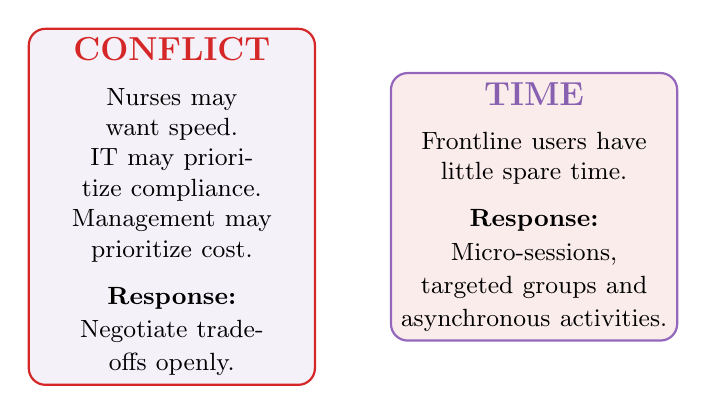
\begin{tikzpicture}

\node[
draw=pdred,thick,rounded corners=6pt,fill=pdpurple!9,
text width=3.4cm,minimum height=2.8cm,align=center
]
(c) at (-4,0)
{
{\large\bfseries\color{pdred}CONFLICT}\\[5pt]
\small Nurses may want speed.\\
IT may prioritize compliance.\\
Management may prioritize cost.\\[6pt]
\textbf{Response:}\\
Negotiate trade-offs openly.
};

\node[
draw=pdpurple,thick,rounded corners=6pt,fill=pdred!9,
text width=3.4cm,minimum height=2.8cm,align=center
]
(t) at (0.6,0)
{
{\large\bfseries\color{pdpurple!90!pdnavy}TIME}\\[5pt]
\small Frontline users have
little spare time.\\[6pt]
\textbf{Response:}\\
Micro-sessions, targeted groups
and asynchronous activities.
};

\end{tikzpicture}

\vspace{.3cm}

{\small\color{pdGrayText}
\textbf{\normalsize Time} management is crucial.
}
\end{frame}

% =========================================================
% 12.3 CONFLICT + TIME + TRUST
% =========================================================
\begin{frame}{Challenges: Conflict, Time, Trust and....}
\centering

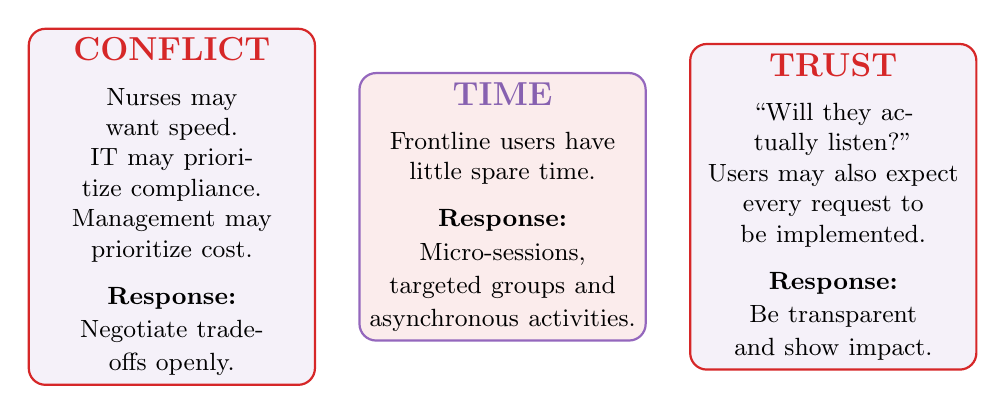
\begin{tikzpicture}

\node[
draw=pdred,thick,rounded corners=6pt,fill=pdpurple!9,
text width=3.4cm,minimum height=2.8cm,align=center
]
(c) at (-4.2,0)
{
{\large\bfseries\color{pdred}CONFLICT}\\[5pt]
\small Nurses may want speed.\\
IT may prioritize compliance.\\
Management may prioritize cost.\\[6pt]
\textbf{Response:}\\
Negotiate trade-offs openly.
};

\node[
draw=pdpurple,thick,rounded corners=6pt,fill=pdred!9,
text width=3.4cm,minimum height=2.8cm,align=center
]
(t) at (0,0)
{
{\large\bfseries\color{pdpurple!90!pdnavy}TIME}\\[5pt]
\small Frontline users have
little spare time.\\[6pt]
\textbf{Response:}\\
Micro-sessions, targeted groups
and asynchronous activities.
};

\node[
draw=pdred,thick,rounded corners=6pt,fill=pdpurple!9,
text width=3.4cm,minimum height=2.8cm,align=center
]
(r) at (4.2,0)
{
{\large\bfseries\color{pdred}TRUST}\\[5pt]
\small ``Will they actually listen?''\\
Users may also expect every
request to be implemented.\\[6pt]
\textbf{Response:}\\
Be transparent and show impact.
};

\end{tikzpicture}

\vspace{.3cm}

{\small\color{pdGrayText}
\textbf{\normalsize Designers} are to respect clients' expectations.
\textit{\normalsize Stakeholders} must trust the skills of designers.
}
\end{frame}

% =========================================================
% 13. PRIVACY
% =========================================================
\begin{frame}{Challenge IV: Participation vs. Privacy}
\centering

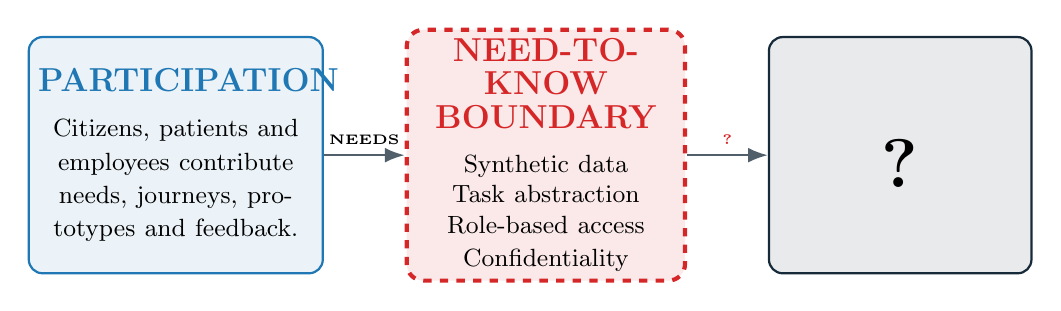
\begin{tikzpicture}

\node[
draw=pdblue,thick,rounded corners=5pt,fill=pdblue!9,
text width=3.5cm,minimum height=3cm,align=center
]
(p) at (-4.7,0)
{
{\large\bfseries\color{pdblue}PARTICIPATION}\\[4.3pt]
\small Citizens, patients and employees
contribute needs, journeys,
prototypes and feedback.
};

\node[
draw=pdred,dashed,line width=1.5pt,rounded corners=6pt,
fill=pdred!10,text width=3.3cm,
minimum height=3cm,align=center
]
(b) at (0,0)
{
{\large\bfseries\color{pdred}NEED-TO-KNOW}\\
{\large\bfseries\color{pdred}BOUNDARY}\\[5pt]
\small Synthetic data\\
Task abstraction\\
Role-based access\\
Confidentiality
};

\node[
draw=pdnavy,thick,rounded corners=5pt,fill=pdnavy!10,
text width=3.1cm,minimum height=3cm,align=center
]
(x) at (4.5,0)
{
{\large\bfseries }\\[5pt]
\Huge \textbf{?}
};

\draw[arrow](p)--node[above,font=\tiny\bfseries]{NEEDS}(b);
\draw[arrow](b)--node[above,font=\tiny\bfseries,text=pdred]
{?}(x);

\end{tikzpicture}

\vspace{.3cm}

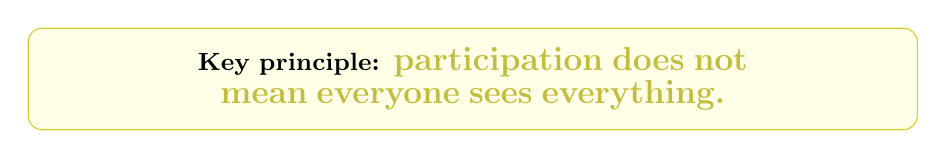
\begin{tikzpicture}
\node[
draw=yellow!80!pdnavy,fill=yellow!10,
rounded corners=5pt,text width=10.8cm,
align=center,inner sep=7pt
]
{\small\bfseries
Key principle:
\textcolor{yellow!70!pdnavy}
{\large participation does not mean everyone sees everything.}};
\end{tikzpicture}

\end{frame}

% =========================================================
% 14. STRUCTURED PARTICIPATION
% =========================================================
\begin{frame}{Ensuring Confidentiality}
\centering


\begin{tikzpicture}

\node[
draw=pdblue,thick,rounded corners=5pt,fill=pdblue!9,
text width=3.5cm,minimum height=2cm,align=center
]
(p) at (-4.7,0)
{
{\large\bfseries\color{pdblue}PARTICIPATION}\\[4.3pt]
};

\node[
draw=pdred,dashed,line width=1.5pt,rounded corners=6pt,
fill=pdred!10,text width=3.3cm,
minimum height=2cm,align=center
]
(b) at (0,0)
{
{\large\bfseries\color{pdred}NEED-TO-KNOW}\\
{\large\bfseries\color{pdred}BOUNDARY}\\[5pt]
\small Synthetic data\\
};

\node[
draw=pdnavy,thick,rounded corners=5pt,fill=pdnavy!10,
text width=3.1cm,minimum height=3cm,align=center
]
(x) at (4.5,0)
{
{\large\bfseries RESTRICTED CORE}\\[5pt]
\small Raw medical records\\
Classified databases\\
Proprietary algorithms\\
Credentials
};

\draw[arrow](p)--node[above,font=\tiny\bfseries]{NEEDS}(b);
\draw[arrow](b)--node[above,font=\tiny\bfseries,text=pdred]
{SHIELDED}(x);

\end{tikzpicture}

\vspace{.3cm}


\begin{tikzpicture}

\node[
font=\large\bfseries,align=center,text=pdgreen
] at (0,-3)
{
Participation can be broad in \textit{purpose}\\
while access remains narrow in \textit{scope}.
};

\end{tikzpicture}
\end{frame}

% =========================================================
% 15. CONCLUSION
% =========================================================
\begin{frame}{Conclusion: A Change in the Design Paradigm}
\centering

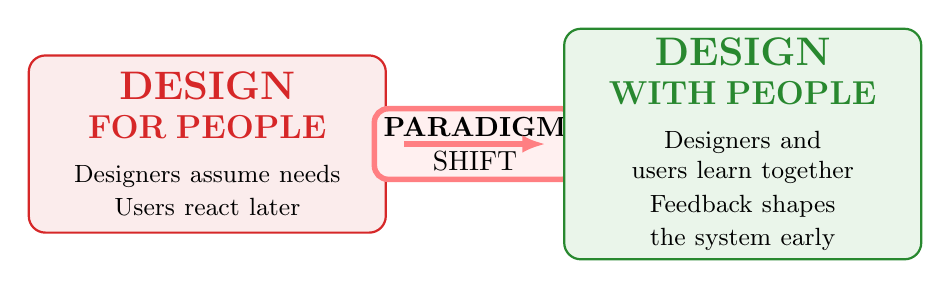
\begin{tikzpicture}

\node[
draw=pdred,thick,rounded corners=6pt,fill=pdred!9,
text width=4.3cm,minimum height=2.25cm,align=center
]
(for) at (-3.4,.5)
{
{\Large\bfseries\color{pdred}DESIGN}\\[2pt]
{\large\bfseries\color{pdred}FOR PEOPLE}\\[5pt]
\small Designers assume needs\\
Users react later
};

\node[
draw=pdorange,line width=2pt,rounded corners=5pt,
fill=pdorange!12,minimum width=2.4cm,
minimum height=.75cm,align=center
] at (0,.5)
{\bfseries PARADIGM\\SHIFT};

\node[
draw=pdgreen!80!pdnavy,thick,rounded corners=6pt,
fill=pdgreen!10,text width=4.3cm,
minimum height=2.25cm,align=center
]
(with) at (3.4,.5)
{
{\Large\bfseries\color{pdgreen!80!pdnavy}DESIGN}\\[2pt]
{\large\bfseries\color{pdgreen!80!pdnavy}WITH PEOPLE}\\[5pt]
\small Designers and users learn together\\
Feedback shapes the system early
};

\draw[-{Latex[length=3mm]},pdorange,line width=2pt]
(-.9,.5)--(.9,.5);

\end{tikzpicture}

\vspace{.4cm}


\begin{tikzpicture}

\node[pill=pdblue,minimum width=2.7cm, minimum height=.75cm]
(s){STAKEHOLDERS};

\node[pill=pdorange,minimum width=2.7cm,minimum height=.75cm,
right=.5cm of s]
(i){INSIGHT};

\node[pill=pdgreen,minimum width=2.7cm, minimum height=.75cm,
right=.5cm of i]
(c){CO-DESIGN};

\node[pill=pdnavy,minimum width=3cm, minimum height=.75cm, 
right=.5cm of c]
(v){ENDURING VALUE};

\draw[arrow](s)--(i);
\draw[arrow](i)--(c);
\draw[arrow](c)--(v);

\end{tikzpicture}

\end{frame}

% =========================================================
% 16. FINAL TAKEAWAY
% =========================================================
\begin{frame}[plain]

\begin{tikzpicture}[remember picture,overlay]

\fill[pdnavy]
(current page.south west) rectangle
(current page.north east);

\node[anchor=center,yshift=1cm] at (current page.center)
{
\begin{minipage}{12.5cm}
\centering
{\small\color{pdorange}\bfseries THE CENTRAL TAKEAWAY}\\[12pt]

{\Huge\bfseries\color{white}
DESIGN FOR PEOPLE}\\[7pt]

{\Large\color{pdfooter}becomes}\\[7pt]

{\Huge\bfseries\color{pdorange}
DESIGN WITH PEOPLE}
\end{minipage}
};

\node[
anchor=center,yshift=-1.5cm,
text width=11.5cm,align=center
] at (current page.center)
{
\large\itshape\color{pdCream}
``Participatory Design gives the people affected by a system
a meaningful voice in shaping it.''
};

\node[
anchor=south,yshift=.8cm,text=white,
font=\scriptsize\bfseries
] at (current page.south)
{
CSE200 \quad\textcolor{pdorange}{\textbullet}\quad
Participatory Design
};

\end{tikzpicture}
\end{frame}

% =========================================================
% 17. THANK YOU
% =========================================================
\begin{frame}[plain]

\begin{tikzpicture}[remember picture,overlay]

\fill[pdCream]
(current page.south west) rectangle
(current page.north east);

\node[
anchor=center,
yshift=1cm,
text=pdnavy,
align=center
] at (current page.center)
{
{\Huge\bfseries THANK YOU}\\[8pt]

{\Large\color{pdnavy}
for listening}
};

\draw[
pdnavy,
line width=1.5pt
]
([xshift=-2.5cm,yshift=-.35cm]current page.center) --
([xshift=2.5cm,yshift=-.35cm]current page.center);


\node[
anchor=south,
yshift=.8cm,
text=pdfooter,
font=\scriptsize\bfseries
] at (current page.south)
{
\small\color{pdnavy}\bfseries CSE23-B1-Group7 \quad\textcolor{pdnavy}{\textbullet}
\small\color{pdnavy}\bfseries
CSE200 \quad\textbullet\quad PARTICIPATORY DESIGN
};

\end{tikzpicture}
\end{frame}
\end{document}